% \documentclass[review]{vgtc}
\documentclass{vgtc}
\usepackage{amsmath,amsfonts}
\usepackage{algorithmic}
\usepackage{algorithm}
\usepackage{booktabs}
\usepackage[table]{xcolor}
\usepackage{array}
\usepackage{textcomp}
\usepackage{stfloats}
\usepackage{url}
\usepackage{verbatim}
\usepackage{graphicx}
\usepackage{cite}
\usepackage{comment}
\usepackage{soul}
\usepackage{transparent}
\usepackage[svgnames]{xcolor}
\usepackage{tcolorbox}
\usepackage{setspace}
\usepackage{tikz}
\usepackage{amssymb}
\usepackage{fancyhdr}
\usetikzlibrary{calc,positioning,arrows.meta}
\usepackage{wrapfig}
\usepackage{endnotes}
\usepackage{minted}
\usepackage{multirow}
\usepackage{xcolor, colortbl}
% \usepackage[colorinlistoftodos]{todonotes}
\definecolor{OliveGreen}{RGB}{183, 207, 178}
\definecolor{DarkYellow}{HTML}{DEA601}
\definecolor{DarkOrange}{HTML}{ED7D31}
\definecolor{DarkBlue}{HTML}{4472C4}
\usepackage{xspace}
\newcommand{\taskWhy}{\textit{\textbf{\textcolor{DarkOrange}{Why?}}}\xspace}
\newcommand{\taskHow}{\textit{\textbf{\textcolor{DarkBlue}{How?}}}\xspace}
\newcommand{\taskWhat}{\textit{\textbf{\textcolor{DarkYellow}{What?}}}\xspace}

\newcommand*\rot{\rotatebox{90}}
\newcommand{\nonterm}[1]{\textbf{\textsf{#1}}}
\newcommand{\literal}[1]{\texttt{#1}}
\newcommand{\typeval}[1]{\textit{#1}}
\newcommand{\dictkey}[1]{\texttt{\textcolor{black}{#1}}}
\renewcommand{\arraystretch}{0.99} % Increase row height for better readability



\definecolor{tsblue}{HTML}{2C3E50}   % for \nonterm
\definecolor{tsteal}{HTML}{2F855A}   % for \literal
\definecolor{tsorange}{HTML}{C05621} % for \typeval

\renewcommand{\nonterm}[1]{\textbf{\textcolor{tsblue}{\textsf{#1}}}}
\renewcommand{\literal}[1]{\textcolor{tsteal}{\texttt{#1}}}
\renewcommand{\typeval}[1]{\textcolor{tsorange}{\textit{#1}}}

\newcommand{\optdefeq}{\stackrel{\text{opt}}{\mathrel{:=}}}
\newcommand{\defeq}{\mathrel{:=}}
\newcommand{\alt}{\;|\;}
\newcommand{\sep}{,\;}
\newcommand{\seq}[1]{\langle{}#1\rangle{}}

% \usepackage{caption}
% \setlength{\belowcaptionskip}{2pt}

% \usepackage[compact]{titlesec}
% \titlespacing{\section}{0pt}{0.5ex}{0.5ex} % Adjust these values
% \titlespacing{\subsection}{0pt}{0.5ex}{0.5ex} % Adjust these values

\usepackage[compact]{titlesec}
\titlespacing{\section}{0pt}{1ex}{0ex}
\titlespacing{\subsection}{0pt}{1ex}{0ex}


\setstretch{0.95}
\setlength{\abovecaptionskip}{7pt}
% \setlength{\belowcaptionskip}{5pt}

% \setlength{\parskip}{0pt}
% \setlength{\parindent}{0pt}
\setlength{\belowcaptionskip}{-7pt}

% \setlength{\parskip}{0.5em}

\setlength{\parindent}{0.7em}  % restore indent for normal paragraphs

\makeatletter
\renewcommand\section{\@startsection{section}{1}{\z@}%
  {-2ex \@plus -1ex \@minus -.2ex}%
  {0.8ex \@plus .2ex}%
  {\@afterindentfalse\reset@font\normalsize\sffamily\bfseries\scshape\vgtc@sectionfont}}

\renewcommand\subsection{\@startsection{subsection}{2}{\z@}%
  {-1.8ex\@plus -1ex \@minus -.2ex}%
  {0.8ex \@plus .2ex}%
  {\@afterindentfalse\reset@font\normalsize\sffamily\bfseries\vgtc@sectionfont}}

\renewcommand\subsubsection{\@startsection{subsubsection}{3}{\z@}%
  {-1.8ex\@plus -1ex \@minus -.2ex}%
  {0.8ex \@plus .2ex}%
  {\@afterindentfalse\reset@font\sffamily\normalsize\vgtc@sectionfont}}
\makeatother






% latin
\newcommand{\etal}{et al.\xspace}
\newcommand{\etals}{\etal{}'s}
\newcommand{\ie}{{i.e.,}}
\newcommand{\eg}{{e.g.,}}
\newcommand{\etc}{{etc.}}
\newcommand{\cf}{{cf.}}
\newcommand{\ala}{\`a la}



% fancy refs
\newcommand{\figref}[1]{\hyperref[#1]{Fig.~\ref*{#1}}}
\newcommand{\secref}[1]{\hyperref[#1]{Sec.~\ref*{#1}}}

\newcommand{\parahead}[1]
{%
    \vspace{0.07in}%
    \noindent%
    \textbf{\textit{#1.}}%
}

\newcommand{\parasubhead}[1]
{%
    % \vspace{0.07in}%
    \textit{#1.}%
}



% highlighting

\newcommand{\hlc}[2][yellow]{{%
                  \colorlet{foo}{#1}%
                  \sethlcolor{foo}\hl{#2}}%
}
\definecolor{quoteColor}{HTML}{C46299}
\newcommand\qt[1]{\hlc[quoteColor!30]{``#1''}}
\newcommand{\pxx}[1]{\textbf{P$_{#1}$}}

\usepackage[normalem]{ulem}
% \usepackage{lmodern} % fix the sc font issue
\definecolor{linkColor}{HTML}{257E98}
\setuldepth{Berlin}
\newcommand\asLink[2]{\textcolor{linkColor}{\small\href{#1}{\ul{#2}}}}
% \newcommand\asLink[2]{\textcolor{linkColor}{\small$<$\href{#1}{\ul{#2}}$>$}}

% \newcommand{\osf}{\asLink{https://osf.io/d8bxr}{osf.io/d8bxr}}

% stuff that was already in the doc


%% Custom in-doc communication commands
% \newcommand{\com}[1]{\textbf{\textit{[#1]}}}
\newcommand{\com}[1]{[#1]}
% \newcommand{\com}[1]{}
\newcommand{\fix}[1]{\textcolor{red}{\com{#1}}}
\newcommand{\pr}[1]{\textcolor{blue}{\com{PR: #1}}}
\newcommand{\rz}[1]{\textcolor{teal}{\com{Rahat: #1}}}
\newcommand{\am}[1]{\textcolor{red}{\com{AM: #1}}}
\newcommand{\dl}[1]{\textcolor{violet}{\com{Dil: #1}}}
% \newcommand{\fix}[1]{\textcolor{red}{}}
% \newcommand{\pr}[1]{\textcolor{blue}{}}
% \newcommand{\rz}[1]{\textcolor{teal}{}}
% \newcommand{\am}[1]{\textcolor{red}{}}
% \newcommand{\dl}[1]{\textcolor{violet}{}}

\newcommand{\para}[1]{\vspace{0.15cm}\noindent\textbf{#1}}

\newcommand{\greyCircle}[1]{%
\tikz[baseline=(char.base)]{
\node[shape=circle,draw,inner sep=0.4pt,fill=gray!25] (char) {#1};}%
}





%% Custom Util Commands
\newcommand{\figureautorefname}{Fig.}
\newcommand{\sectionautorefname}{Sect.}
\newcommand{\subsectionautorefname}{\sectionautorefname}
\newcommand{\subsubsectionautorefname}{\sectionautorefname}
\newcommand{\anonymize}[2]{$<$\textit{#1}$>$}
\renewcommand{\paragraph}[1]{\textbf{#1:}}


\definecolor{indvHigh}{HTML}{9BB2E0}
\definecolor{indvMed}{HTML}{C8D6ED}
\definecolor{indvLow}{HTML}{ECF2F9}

\definecolor{grpHigh}{HTML}{B6E09B}
\definecolor{grpMed}{HTML}{D6EDC7}
\definecolor{grpLow}{HTML}{F2F9ED}

\definecolor{ensTaskHigh}{HTML}{B86029}
\definecolor{ensTaskMed}{HTML}{EAB38B}
\definecolor{ensTaskMedLow}{HTML}{EFCAB0}
\definecolor{ensTaskLow}{HTML}{F8E4D8}

\definecolor{ensTotHigh}{HTML}{B7912F}
\definecolor{ensTotMed}{HTML}{F5C242}
\definecolor{ensTotMedLow}{HTML}{F8DA78}
\definecolor{ensTotLow}{HTML}{FDF3D0}

\definecolor{dsHigh}{HTML}{2F5597}
\definecolor{dsMed}{HTML}{8FAADC}
\definecolor{dsLow}{HTML}{B4C7E7}
\onlineid{1199}

%% In preprint mode you may define your own headline. If not, the default IEEE copyright message will appear in preprint mode.
%\preprinttext{To appear in IEEE Transactions on Visualization and Computer Graphics.}

%% In preprint mode, this adds a link to the version of the paper on IEEEXplore
%% Uncomment this line when you produce a preprint version of the article 
%% after the article receives a DOI for the paper from IEEE
%\ieeedoi{xx.xxxx/TVCG.201x.xxxxxxx}

%% declare the category of your paper, only shown in review mode
\vgtccategory{Application}

%% please declare the paper type of your paper to help reviewers, only shown in review mode
%% choices:
%% * algorithm/technique
%% * application/design study
%% * evaluation
%% * system
%% * theory/model
\vgtcpapertype{application}

%% Paper title.
\title{Site Accessibility Auditor: Browser-Integrated Accessibility Auditing for Interactive and Visualization-Rich Web Pages}

%% Author ORCID IDs should be specified using \authororcid like below inside
%% of the \author command. ORCID IDs can be registered at https://orcid.org/.
%% Include only the 16-digit dashed ID.
\author{%
  \authororcid{Md Rahat-uz- Zaman}{0000-0001-6728-7569}, 
  and \authororcid{Paul Rosen} {0000-0002-0873-9518}
}

% \authorfooter{
%   %% insert punctuation at end of each item
%   \item
%   	Josiah Carberry is with Brown University.
%   	E-mail: jcarberry@example.com
%   \item
%   	Ed Grimley is with Grimley Widgets, Inc.
%   	E-mail: ed.grimley@example.com.

%   \item Martha Stewart is with Martha Stewart Enterprises at Microsoft
%   Research.
%   	E-mail: martha.stewart@example.com.
% }

%% Abstract section.
\abstract{Automated web accessibility tools are effective at catching common rule violations, but they often provide limited support for the inspection work developers still need to do inside real interfaces. Problems such as undersized touch targets, confusing keyboard order, chart-specific accessibility gaps, and color-dependent meaning are easier to understand when the evidence remains visible on the page being debugged. We present \textit{Site Accessibility Auditor}, a Chrome DevTools extension that supports this style of inspection through four complementary panels: touch-target auditing for WCAG~2.2 target-size checks, tab-order visualization for keyboard navigation structure, chart detection and inspection for SVG/canvas/image/library-backed visualizations, and an AI-assisted color audit that groups page colors into semantic sections and flags likely color-related risks. Rather than collapsing results into a single score, the system emphasizes page overlays, module-specific representations, and direct inspection in situ. We illustrate the design through three fixture-based scenarios involving a static form, a dashboard-style interface, and a chart-heavy page. Our contribution is a practical browser-integrated workflow for accessibility inspection that better supports interactive and visualization-rich pages than isolated static checks alone.
}

%% Keywords that describe your work. Will show as 'Index Terms' in journal
%% please capitalize first letter and insert punctuation after last keyword
\keywords{accessibility, web auditing, interactive systems, data visualization}

%% A teaser figure can be included as follows
\teaser{
  \centering
  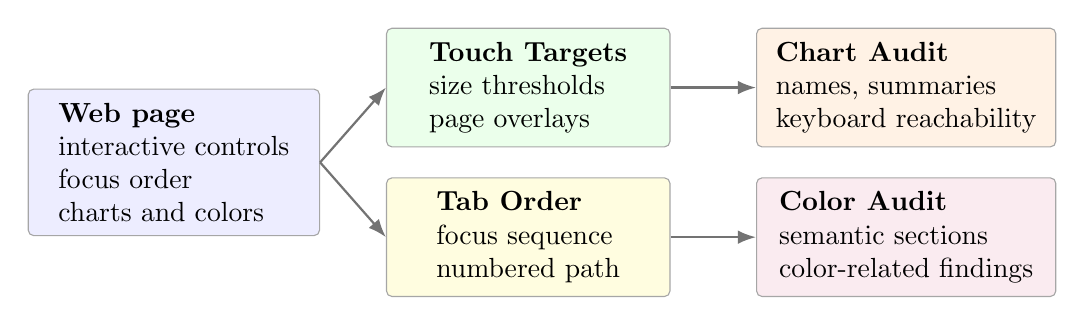
\begin{tikzpicture}[
    x=1cm, y=1cm,
    panel/.style={rounded corners=2pt, draw=black!35, fill=gray!6, minimum height=1.45cm, align=left, inner sep=5pt},
    arrow/.style={-Latex, thick, draw=black!55}
  ]
    \node[panel, fill=blue!7, minimum width=3.7cm] (page) at (0,0) {\textbf{Web page}\\interactive controls\\focus order\\charts and colors};
    \node[panel, fill=green!8, minimum width=3.6cm] (touch) at (4.5,0.95) {\textbf{Touch Targets}\\size thresholds\\page overlays};
    \node[panel, fill=yellow!12, minimum width=3.6cm] (tab) at (4.5,-0.95) {\textbf{Tab Order}\\focus sequence\\numbered path};
    \node[panel, fill=orange!10, minimum width=3.8cm] (chart) at (9.3,0.95) {\textbf{Chart Audit}\\names, summaries\\keyboard reachability};
    \node[panel, fill=purple!8, minimum width=3.8cm] (color) at (9.3,-0.95) {\textbf{Color Audit}\\semantic sections\\color-related findings};

    \draw[arrow] (page.east) -- (touch.west);
    \draw[arrow] (page.east) -- (tab.west);
    \draw[arrow] (touch.east) -- (chart.west);
    \draw[arrow] (tab.east) -- (color.west);
  \end{tikzpicture}
  \caption{The extension organizes accessibility inspection into task-specific DevTools panels rather than a single aggregate score. Each panel preserves the evidence most useful for that class of problem.}
  \label{fig:teaser}
}

%% Uncomment below to disable the manuscript note
%\renewcommand{\manuscriptnotetxt}{}

%% Copyright space is enabled by default as required by guidelines.
%% It is disabled by the 'review' option or via the following command:
%\nocopyrightspace


%%%%%%%%%%%%%%%%%%%%%%%%%%%%%%%%%%%%%%%%%%%%%%%%%%%%%%%%%%%%%%%%
%%%%%%%%%%%%%%%%%%%%%% LOAD PACKAGES %%%%%%%%%%%%%%%%%%%%%%%%%%%
%%%%%%%%%%%%%%%%%%%%%%%%%%%%%%%%%%%%%%%%%%%%%%%%%%%%%%%%%%%%%%%%

%% Tell graphicx where to find files for figures when calling \includegraphics.
%% Note that due to the \DeclareGraphicsExtensions{} call it is no longer necessary
%% to provide the the path and extension of a graphics file:
%% 
\includegraphics{diamondrule} is completely sufficient.
\graphicspath{{figs/}{figures/}{pictures/}{images/}{./}} % where to search for the images

%% Only used in the template examples. You can remove these lines.
\usepackage{tabu}                      % only used for the table example
\usepackage{booktabs}                  % only used for the table example
\usepackage{lipsum}                    % used to generate placeholder text
\usepackage{mwe}                       % used to generate placeholder figures
\usepackage{wasysym}

\usepackage{svg}


%% We encourage the use of mathptmx for consistent usage of times font
%% throughout the proceedings. However, if you encounter conflicts
%% with other math-related packages, you may want to disable it.
\usepackage{mathptmx}                  % use matching math font

\begin{document}

%%%%%%%%%%%%%%%%%%%%%%%%%%%%%%%%%%%%%%%%%%%%%%%%%%%%%%%%%%%%%%%%
%%%%%%%%%%%%%%%%%%%%%% START OF THE PAPER %%%%%%%%%%%%%%%%%%%%%%
%%%%%%%%%%%%%%%%%%%%%%%%%%%%%%%%%%%%%%%%%%%%%%%%%%%%%%%%%%%%%%%%

%% The ``\maketitle'' command must be the first command after the
%% ``\begin{document}'' command. It prepares and prints the title block.
%% the only exception to this rule is the \firstsection command
% \firstsection{Introduction}

\maketitle


%% \section{Introduction} %for journal use above \firstsection{..} inste
\section{Introduction}
\label{sec:introduction}

Web accessibility evaluation remains caught between two incomplete modes of practice. On one side, automated tools quickly surface common failures such as missing labels, invalid ARIA, or contrast errors. On the other side, experienced auditors still need to manually inspect interaction patterns, focus behavior, and state-dependent interface changes that are difficult to formalize or automate. W3C guidance explicitly cautions that no single tool can determine whether a site is accessible, and prior work has shown the harm of relying on automated checks alone~\cite{w3cEvalOverview,vigo2013benchmarking}. The continuing prevalence of accessibility failures on popular websites underscores the practical importance of this gap~\cite{webaim2026}.

This gap is widening as web interfaces become more interactive and visually dense. WCAG~2.2 adds requirements that are especially relevant to contemporary web applications, including target size, focus visibility, and input patterns that are often state-dependent~\cite{wcag22rec,wcag22new}. At the same time, visualization research has shown that charts demand richer accessibility support than a basic alt text or table link, because readers need structure, navigation, and description to explore data non-visually~\cite{zong2022rich,blanco2022olli}. Yet the dominant browser-based auditing workflows remain largely page-static and checklist-oriented.

We argue that accessibility auditing for modern web applications should be treated as an inspection problem as much as a detection problem. Auditors need representations that keep geometric evidence, keyboard structure, color usage, and chart metadata close to the live page they are debugging. To support this workflow, we developed \textit{Site Accessibility Auditor}, a Chrome DevTools extension that brings several focused audit views into a single browser-integrated environment.

The paper makes three contributions. First, we present a systems design for \textit{browser-integrated accessibility inspection} inside DevTools, built around complementary panels for touch targets, tab order, charts, and color usage. Second, we introduce a \textit{visualization-aware audit workflow} that treats charts as explicit audit targets rather than generic images, surfacing risks such as missing names, absent summaries, limited keyboard reachability, and likely color-only encodings. Third, we show how \textit{AI-assisted color semantics} can complement deterministic inspection by grouping page colors into meaningful sections and flagging likely accessibility risks without replacing the underlying page evidence. Rather than claiming full automation, our goal is to provide a practical environment that helps developers and researchers inspect accessibility problems that static scans under-represent.


\section{Background and Related Work}
\label{sec:related}

\parahead{Automated accessibility evaluation.}
Accessibility evaluation tools are widely used because they efficiently identify machine-detectable barriers and integrate well with authoring and development workflows~\cite{w3cToolsOverview,w3cEvalOverview}. However, their limits are well established. Vigo \etal{} found that sole reliance on automated testing can leave substantial WCAG coverage unexamined and can also introduce false positives~\cite{vigo2013benchmarking}. W3C's ACT effort aims to harmonize how rules are specified and interpreted, but ACT rules still span automated, semi-automated, and manual procedures~\cite{w3cActOverview}. Our work does not attempt to replace rule engines; instead, it emphasizes inspection-oriented representations that help developers interpret accessibility evidence directly inside DevTools.

\parahead{Inspection of interactive interfaces.}
Recent WCAG~2.2 additions make clear that accessibility problems increasingly arise from interaction mechanics rather than static markup alone~\cite{wcag22rec,wcag22new}. Failures involving small targets, confusing keyboard order, or ambiguous visual encoding often require an analyst to inspect geometry, sequence, and page context rather than simply read a checklist result. Existing browser-integrated tools such as Lighthouse are valuable baselines, but they remain oriented around page-level pass/fail summaries~\cite{lighthouseOverview,lighthouseA11y}. Our system therefore focuses on representations that make these interaction-relevant properties easier to inspect in place.

\parahead{Accessible data visualization.}
Visualization research has shown that charts require richer non-visual access than a short label or fallback table alone. Rich screen reader experiences depend on structural organization, navigation mechanisms, and meaningful descriptions~\cite{zong2022rich}. Olli demonstrates one route toward toolkit-agnostic accessible chart structures~\cite{blanco2022olli}. At the same time, W3C guidance on complex images emphasizes the need for both concise identification and longer-form descriptions for charts and other information-dense graphics~\cite{w3cComplexImages}. These findings motivate our chart-focused auditing module, which treats visualizations as distinct audit targets rather than generic DOM elements.

\section{System Design}
\label{sec:system}

\begin{figure}[t]
  \centering
  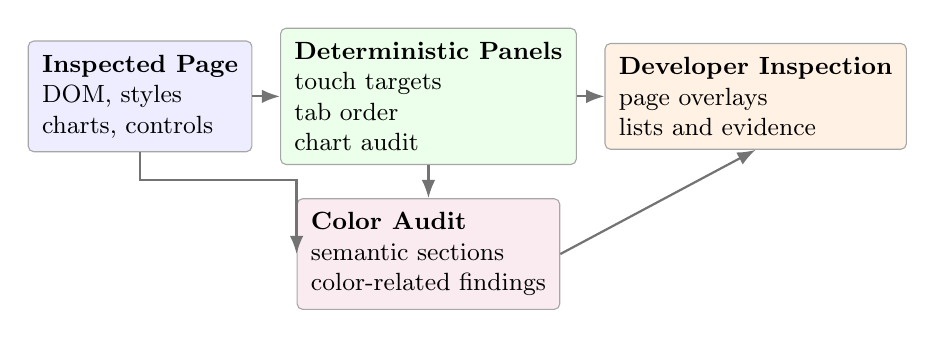
\begin{tikzpicture}[
    node distance=0.5em,
    font=\small,
    box/.style={rounded corners=2pt, draw=black!35, fill=gray!7, minimum width=0.205\linewidth, minimum height=1.15cm, align=left, inner sep=5pt},
    arrow/.style={-Latex, thick, draw=black!55}
  ]
    \node[box, fill=blue!7] (page) {\textbf{Inspected Page}\\DOM, styles\\charts, controls};
    \node[box, fill=green!8, right=0.35cm of page] (modules) {\textbf{Deterministic Panels}\\touch targets\\tab order\\chart audit};
    \node[box, fill=orange!10, right=0.35cm of modules] (workflow) {\textbf{Developer Inspection}\\page overlays\\lists and evidence};
    \node[box, fill=purple!8, below=0.42cm of modules] (llm) {\textbf{Color Audit}\\semantic sections\\color-related findings};

    \draw[arrow] (page) -- (modules);
    \draw[arrow] (modules) -- (workflow);
    \draw[arrow] (modules) -- (llm);
    \draw[arrow] (page.south) -- ++(0,-0.35) -| (llm.west);
    \draw[arrow] (llm.east) -- (workflow.south);
  \end{tikzpicture}
  \caption{System overview. The extension keeps accessibility inspection inside DevTools by combining deterministic panels for touch targets, keyboard order, and chart structure with an AI-assisted color audit.}
  \label{fig:architecture}
\end{figure}

The extension is implemented as a Manifest~V3 Chrome DevTools extension with four task-focused panels: touch targets, tab order, color audit, and data visualizations. Rather than routing every finding through a single summary screen, the system gives each auditing problem a representation matched to the evidence a developer needs to inspect.

\parahead{Panel-specific representations.}
The design choice is deliberate. Touch targets are best understood as rectangles and size thresholds; keyboard flow is best understood as an ordered path through focusable elements; charts are best understood as structured objects with labels, captions, legends, and interaction affordances; and page colors benefit from semantic grouping that helps an analyst reason about repeated palette use. Preserving these panel-specific views produces more interpretable evidence than flattening everything into a single list.

\parahead{Deterministic audit modules.}
The first layer of the system performs rule-based inspection over the rendered page. The touch-target module checks interactive elements against WCAG~2.2 target-size thresholds and overlays failures directly on the page. The tab-order module extracts focusable elements, reconstructs keyboard order, identifies positive \literal{tabindex} usage, and visualizes tab paths as numbered overlays. The chart module detects SVG, canvas, image, and library-backed visualization containers, then inspects them for missing accessible names, absent captions or table fallbacks, weak keyboard reachability, and structural cues suggesting color-only encodings.

\parahead{AI-assisted color audit.}
We use an OpenAI client as a narrow semantic layer for color inspection. Rather than asking the model to judge overall accessibility, we restrict it to grouping extracted page colors into human-readable sections and flagging likely color-related risks such as low-contrast clusters, color-only meaning, confusable palettes, and weak interactive-state differentiation. This makes the AI component additive rather than authoritative: it helps organize and interpret page color usage, while the inspected page remains the grounding context.

\begin{table}[t]
\centering
\small
\setlength{\tabcolsep}{3pt}
\begin{tabular}{p{0.18\linewidth} p{0.23\linewidth} p{0.5\linewidth}}
\toprule
\textbf{Module} & \textbf{Primary evidence} & \textbf{Representative output} \\
\midrule
Touch targets & bounding boxes, target sizes & WCAG~2.2 target-size failures and warnings rendered directly on the page \\
Tab order & focusable DOM order, \literal{tabindex}, element rectangles & keyboard path visualization, positive-\literal{tabindex} warnings, programmatic-focus flags \\
Chart audit & renderer type, label, caption, legend items, keyboard affordances & missing chart name, missing summary/table fallback, likely color-only encoding \\
Color audit & extracted DOM colors plus element/context metadata & semantic color sections and likely color-related accessibility findings \\
\bottomrule
\end{tabular}
\caption{Audit modules and evidence types in the current extension.}
\label{tab:modules}
\end{table}

\parahead{Inspection workflow.}
The primary workflow is intentionally simple. An analyst opens the panel that matches the question at hand, runs the corresponding scan, and inspects the resulting evidence directly against the page. The touch-target and tab-order panels emphasize geometric overlays; the chart panel emphasizes detected visualization structure and metadata; the color panel emphasizes grouped palette usage and color-related findings. In practice, developers move among these views as they refine a diagnosis.

This workflow matters because accessibility debugging is rarely linear. Developers alternate between broad questioning and narrow inspection: Is the problem geometric, keyboard-related, chart-specific, or color-dependent? A multi-panel DevTools design supports that shift better than a single undifferentiated results list.

\section{Demonstration Scenarios}
\label{sec:scenarios}

We designed three local fixture pages to exercise the extension's workflow. These fixtures are not presented as a formal evaluation; rather, they illustrate the kinds of evidence the system is designed to surface.

\parahead{Static form fixture.}
A simple page with undersized toolbar controls, a color-only status indicator, and out-of-order positive \literal{tabindex} values exposes the complementarity of the modules. The touch-target panel immediately highlights controls that fail the 24~CSS pixel minimum. The tab-order panel reveals a focus sequence that does not match DOM order. The color audit groups repeated palette use and highlights the status indicator as a likely place where color is carrying meaning by itself.

\parahead{Dynamic dashboard fixture.}
The second fixture includes a disclosure panel, status chips, and dense navigation controls. Here the system is useful not because it automatically explores the page, but because the analyst can open the relevant interface state and then inspect it with the appropriate panel. The tab-order panel reveals whether the disclosed controls join the keyboard sequence coherently, while the color audit helps separate decorative palette choices from status colors that may need redundant non-color encoding.

\parahead{Chart fixture.}
The third fixture contains an SVG bar chart and a canvas chart-like element with limited metadata. The chart module detects both as visualization targets, then flags missing accessible naming, absent summary or table fallback, and weak keyboard affordances. It also surfaces cues suggesting that the visualization may rely on color channels without sufficient labeling. This scenario demonstrates why visualization-aware auditing deserves dedicated treatment rather than being folded into generic image checks.

\parahead{Artifact support.}
The implementation also includes local fixture pages and benchmark scripts, which help position the project as a reusable research artifact rather than a one-off demo. The fixtures support repeatable walkthroughs of touch-target, keyboard-flow, color, and chart issues, and they provide a concrete starting point for future comparative evaluation against baseline tools.

\section{Discussion}
\label{sec:discussion}

The design of \textit{Site Accessibility Auditor} reflects a shift away from monolithic page scores and toward evidence-centered inspection. We do not argue that every accessibility problem should be automatically detected. Instead, we argue that accessibility tooling should help developers \emph{inspect} issues that unfold across geometry, keyboard structure, color usage, and visualization content. In this sense, the system aligns accessibility auditing with long-standing visual analytics ideas: choose representations that fit the question, keep evidence close to source context, and support fast movement between page and panel.

The chart module is particularly important for VIS audiences. While the broader accessibility ecosystem already has mature rule engines for generic HTML failures, visualization-heavy interfaces remain a weak point in everyday development workflows. Our extension contributes a practical bridge between accessible visualization research and browser-based auditing practice by making charts explicit audit entities, surfacing structural risks, and attaching stateful evidence to them.

\parahead{Research utility.}
Beyond end-user utility, the project is designed to support future VIS and accessibility studies. The module structure makes it possible to compare how different representations affect inspection behavior: geometric overlays for touch targets, ordered paths for keyboard flow, structured metadata for charts, and AI-assisted grouping for page colors. This creates a path toward evaluating not only detection coverage but also analyst performance, such as time-to-diagnosis and confidence in interpreting the evidence.

\parahead{Design implications.}
The system suggests three design implications for future accessibility tools. First, \emph{representations should match the evidence}. Geometric thresholds, keyboard sequences, and chart structure are different problems and benefit from different views. Second, \emph{AI assistance should stay narrow and interpretable}. Restricting the semantic layer to color organization and color-related findings keeps its role legible to the user. Third, \emph{visualization interfaces merit dedicated audit representations}. Charts carry structure, legends, interaction affordances, and explanatory text that are poorly captured by generic image-oriented checks.

\parahead{What this enables next.}
Because the repository includes fixtures and benchmark scripts, the project is positioned to support several immediate next steps. One is a comparative benchmark against browser-integrated baselines for touch targets, keyboard order, and chart-related findings. Another is a controlled user study comparing these panel-specific views against more generic issue lists. A third is a chart-focused evaluation using pages from dashboards, journalism, and scientific web applications. We view the current system as an enabling artifact for these studies rather than their final substitute.

The current system also has clear limitations. It does not automate deep exploration of application state, so analysts must still navigate to the interface condition they want to inspect. The AI layer is intentionally narrow and can still produce incomplete or weak interpretations, so it should not be treated as a conformance oracle. Finally, this paper reports a systems contribution and demonstration, not a user study or benchmark comparison. The repository includes fixture pages and benchmarking scripts to support future comparative evaluation against tools such as Lighthouse, but such evaluation remains future work.

\section{Evaluation Agenda}
\label{sec:evaluation}

Although this short paper focuses on system design, the implementation was built to support a concrete evaluation agenda. We outline that agenda here because it clarifies what kinds of research questions the artifact is meant to answer. In particular, the system is designed to enable three kinds of comparison: generic page auditing versus panel-specific inspection, generic image checks versus chart-aware auditing, and raw DOM color extraction versus AI-assisted color organization.

\parahead{Benchmark construction.}
The repository includes local fixture pages that exercise static controls, dashboard-like layouts, and chart structures. These fixtures form a minimal benchmark seed, but the longer-term goal is to expand them into a corpus of dashboard, journalism, and administration interfaces with known accessibility issues. Because the fixtures are local and reproducible, the same pages can be reused across multiple tool comparisons without rebuilding the task context each time.

\parahead{Tool comparison.}
The most direct comparison is against browser-integrated and rules-based baselines. Here the interesting metric is not simply how many issues each tool reports, but which classes of issues benefit from a panel-specific representation. We expect the extension to be most distinctive for touch-target geometry, keyboard sequence debugging, and visualization-specific findings, while conventional rule engines should remain competitive on generic DOM-level checks.

\parahead{Analyst-centered evaluation.}
The second comparison concerns workflow rather than detection alone. A future user study can ask whether these in-situ panels help developers diagnose problems faster than isolated issue lists or external reports. For example, one might measure time-to-first-actionable-fix, confidence in the diagnosis, or how often analysts need to leave the page context to interpret a result.

\parahead{Semantic-layer evaluation.}
The final comparison concerns the role of AI-assisted color semantics. Here the question is not whether the model replaces accessibility evaluation, but whether semantic grouping and color-related findings improve interpretation over raw lists of extracted colors. In our view, such evaluation should focus on organization quality, perceived usefulness, and failure modes rather than on abstract claims that the model ``finds more issues.''

\section{Conclusion}
\label{sec:conclusion}

We presented \textit{Site Accessibility Auditor}, a Chrome DevTools extension for browser-integrated accessibility inspection. The system combines deterministic checks for touch targets, keyboard flow, and chart structure with an AI-assisted color audit, all delivered through task-specific panels that keep evidence close to the inspected page. We contribute a practical systems design that broadens what developers can inspect inside everyday browser tooling, especially for interactive and visualization-rich interfaces. We hope this work helps frame accessibility auditing as a representational design problem as well as a detection problem.


% \clearpage{}

\setstretch{0.948}
\acknowledgments{
  The authors thank the members of the Visualization Design Lab for discussion and feedback on early versions of the system and paper.}


% \clearpage{}

\bibliographystyle{abbrv-doi-hyperref}
\bibliography{main}


% \clearpage{}

% \input{sections/10-appendix}
\end{document}
